% APAR : s’arrêter avant la commande impossible
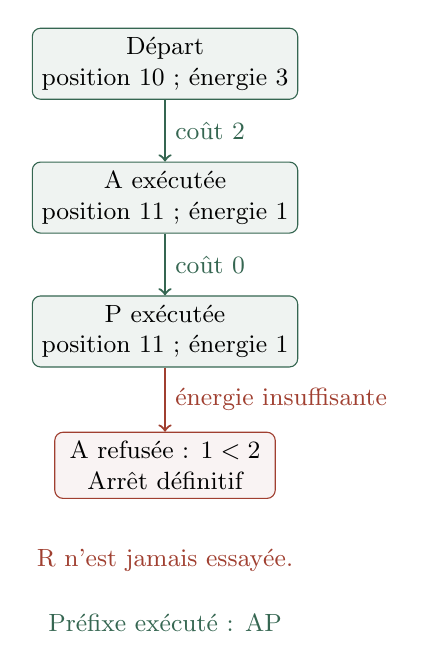
\begin{tikzpicture}[font=\small,
etat/.style={draw,rounded corners=3pt,minimum width=2.8cm,minimum height=0.8cm,align=center},
fleche/.style={->,thick}]
\definecolor{vert}{RGB}{53,102,81}
\definecolor{rouge}{RGB}{160,63,48}
\node[etat,draw=vert,fill=vert!8] (debut) at (0,0) {D\'epart\\position 10 ; \'energie 3};
\node[etat,draw=vert,fill=vert!8] (avance) at (0,-1.7) {A ex\'ecut\'ee\\position 11 ; \'energie 1};
\node[etat,draw=vert,fill=vert!8] (pause) at (0,-3.4) {P ex\'ecut\'ee\\position 11 ; \'energie 1};
\node[etat,draw=rouge,fill=rouge!6] (arret) at (0,-5.1) {A refus\'ee : $1<2$\\Arr\^et d\'efinitif};
\draw[fleche,vert] (debut) -- (avance) node[midway,right] {co\^ut 2};
\draw[fleche,vert] (avance) -- (pause) node[midway,right] {co\^ut 0};
\draw[fleche,rouge] (pause) -- (arret) node[midway,right] {\'energie insuffisante};
\node[align=center,text=rouge] at (0,-6.3) {R n'est jamais essay\'ee.};
\node[align=center,text=vert] at (0,-7.1) {Pr\'efixe ex\'ecut\'e : AP};
\end{tikzpicture}
